% Provenance (never printed): see sources/outline_sources.md (Year 3: the heat
% equation, half-space and plate cooling models, heat flow against age,
% continental geotherms, thermal subsidence). Brief: sources/book5/BRIEFS.md,
% ch. 5. Curves from figdata/bachelor-3/plate_cooling.py (models; Seton et al.
% 2020 age grid and ETOPO1, read only) and continental_geotherm.py.
% Exercise and problem values in the Book 5 scratch calculator calc/ch05.py.
\chapter{النماذج الحرارية للغلاف الصخري}\label{ch:b3:lithosphere-thermal-models}

ابتعد بالسفينة عن ظهرة وسط المحيط فيزداد عمق قاع البحر نحو
\qty{2.5}{km} عند المحور، وأكثر من \qty{5}{km} تحت أقدم
قاع محيطي. لم يُضَف إلى الصفيحة شيء ولم يُنتزع منها، وإنّما بَرَدت فحسب،
وتقلّصت وغاصت. وقاع المحيط مقياسٌ لحرارة الصفيحة التي تحته،
ويقرأ مسبارُ التدفق الحراري المغروس في رواسبه التبريدَ نفسه
من الأعلى. يحلّ هذا الفصل تبريد الصفيحة بطريقتين، بوصفها نصفَ فضاء
وبوصفها صفيحةً ذات سماكةٍ محدودة، ويقارن كلتيهما بعمق
قاع المحيط الحقيقي وتدفقه الحراري، ثم ينتقل إلى القارّات،
التي يأتي جزء من حرارتها من قشرتها نفسها.
% ledger: ps77:depth-age

\begin{recall}
معادلةُ الانتشار للحرارة، $\partial T/\partial t = \kappa\nabla^2T$،
مع الموصلية الحرارية $k$ والانتشارية الحرارية $\kappa =
k/(\rho c)$، تُدرَس في كتب الفيزياء؛ أمّا متسلسلات فورييه ودالة الخطأ
$\operatorname{erf}x = (2/\sqrt\pi)\int_0^xe^{-u^2}\,\mathrm du$ فموجودتان في
مجلّدات الجامعة من كتب الرياضيات. أمّا التدفق الحراري، وإنتاج الحرارة المشعّة،
والمنحنى الحراري، ومقياس الزمن التوصيلي $L^2/\kappa$، والطبقة الحدّية الحرارية
والغلاف الصخري الحراري فقد عُرِّفت في مجلد السنة الأولى،
في فصلها عن ميزانية الحرارة في الأرض؛ والتوازن الأيزوستاتي في فصلها
عن التوازن الأيزوستاتي والشذوذات الثقلية؛ وقانون العمق--العمر $d = d_r + C\sqrt t$ بُرهن في
فصلها عن الشقوق والظهرات والهوامش السلبية، مُسلِّمًا بالمقطع
الحراري الذي يشتقّه هذا الفصل. ونموذج تمدّد الأحواض، والهبوط بعد
التصدّع والثابت الزمني الحراري موجودان في مجلد السنة الثانية، في
فصلها عن الأحواض الرسوبية.
\end{recall}

\section{التوصيل والانتقال الأفقي ونسبتهما}

تنتقل الحرارة في الغلاف الصخري بطريقتين: تنتشر نزولًا على طول تدرّج
درجة الحرارة، وتحملها صخور متحرّكة، كصفيحةٍ مبتعدةٍ عن ظهرة،
وجبلٍ متآكلٍ يرتفع، وصهارةٍ صاعدة. وأيّ الطريقتين تغلب يتوقّف على
عددٍ واحد.

\begin{definition}[عدد بيكليه الحراري]\label{def:b3:lithosphere-thermal-models:peclet}
لصخرٍ يتحرّك بسرعة $u$ عبر طولٍ $L$، يُسمّى \emph{عدد بيكليه
الحراري}\index{عدد بيكليه الحراري} ويُعطى بالعلاقة:
\[
  \mathrm{Pe} = \frac{uL}{\kappa},
\]
وهو نسبةُ الزمن التوصيلي $L^2/\kappa$ إلى زمن الانتقال الأفقي $L/u$.
يغلب الانتقال الأفقي حيث $\mathrm{Pe} \gg 1$، ويغلب التوصيل حيث
$\mathrm{Pe} \ll 1$.
\end{definition}

صفيحةٌ مبتعدةٌ عن ظهرة بسرعة \qty{25}{mm/yr} تملك، على مسافة
\qty{95}{km}، $\mathrm{Pe} \approx 94$ مع $\kappa = \qty{0.8e-6}{m^2.s^{-1}}$:
تُنقل الحرارة جانبيًا بفعل الصفيحة أسرع بكثير من انتشارها جانبيًا.
ولذلك يبرد كلّ عمودٍ رأسيّ من الصفيحة كأنّه منفرد، بالتوصيل الرأسي
إلى قاع البحر البارد، وعمره $t$ يمثّل الزمن منذ أن
غادر المحور. وبذلك تتحوّل مسألة ثنائية البعد إلى مسألة في العمق
والزمن.

\section{نصف الفضاء المبرِّد}

\begin{definition}[نموذج تبريد نصف الفضاء]\label{def:b3:lithosphere-thermal-models:half-space}
يعامِل \emph{نموذج تبريد نصف الفضاء}\index{نموذج تبريد نصف الفضاء} الغلاف الصخري المحيطي
كلَّ عمودٍ بوصفه نصف فضاءٍ $z \ge 0$ ذا انتشاريةٍ منتظمة،
عند درجة الحرارة المنتظمة $T_m$ للوشاح لحظةَ مغادرته
محورَ الظهرة، ويُثبَّت سطحُه منذ ذلك الحين عند درجة الحرارة $T_0$
لقاع البحر، دون إنتاجٍ للحرارة ودون قاعٍ أسفل.
\end{definition}

\begin{theorem}[المنحنى الحراري لدالة الخطأ]\label{thm:b3:lithosphere-thermal-models:erf}
في \omterm{def:b3:lithosphere-thermal-models:half-space}{نموذج تبريد نصف الفضاء}، تكون درجة الحرارة على العمق $z$ تحت
قاع بحرٍ عمرُه $t$ هي:
\[
  T(z, t) = T_0 + (T_m - T_0)\operatorname{erf}\frac{z}{2\sqrt{\kappa t}} .
\]
وهذا هو \emph{المنحنى الحراري لدالة الخطأ}\index{المنحنى الحراري لدالة الخطأ}.
\end{theorem}

\begin{proof}
لتكن $\theta = (T - T_0)/(T_m - T_0)$؛ فهي تحقّق $\partial\theta/\partial t =
\kappa\,\partial^2\theta/\partial z^2$ مع $\theta(z, 0) = 1$ من أجل $z > 0$
و$\theta(0, t) = 0$ من أجل $t > 0$. ليس للمسألة مقياسُ طولٍ خاصّ بها:
إذا كانت $\theta(z, t)$ حلًّا، فكذلك $\theta(\lambda z, \lambda^2t)$ من أجل كلّ
$\lambda > 0$، بالقيم الابتدائية والحدّية نفسها؛ ولمّا كان الحلّ
وحيدًا، فإنّ $\theta$ يعتمد على $z$ و$t$ فقط عبر $\eta = z/(2\sqrt{\kappa
t})$. بكتابة $\theta = f(\eta)$، مع $\partial\eta/\partial t = -\eta/(2t)$
و$\partial\eta/\partial z = 1/(2\sqrt{\kappa t})$,
\[
  -\frac{\eta}{2t}f'(\eta) = \kappa\,\frac{f''(\eta)}{4\kappa t},
  \qquad\text{إذن}\qquad f'' + 2\eta f' = 0 .
\]
ومنه $f' = Ae^{-\eta^2}$ و$f = A\int_0^\eta e^{-u^2}\,\mathrm du + B$.
يعطي الشرط السطحي، عند $\eta = 0$، $B = 0$؛ والشرط الابتدائي، الذي
يتحقّق عند كلّ عمقٍ حين $t \to 0$، أي حين $\eta \to \infty$، فيعطي
$A\sqrt\pi/2 = 1$. إذن $f = \operatorname{erf}\eta$.
\end{proof}

تعتمد درجة الحرارة عند عمقٍ معيّن على $z/\sqrt t$ وحده: يهبط خطّ
متساوي الحرارة بقدر الجذر التربيعي للعمر، وتبلغ سماكة الطبقة المبرّدة عند \qty{40}{Myr} ضعفَ
سُمكها عند \qty{10}{Myr}. ويُستنتَج التدفق الحراري السطحي بالاشتقاق.

\begin{proposition}[علاقة التدفق الحراري--العمر]\label{prop:b3:lithosphere-thermal-models:heat-flow}
في \omterm{def:b3:lithosphere-thermal-models:half-space}{نموذج تبريد نصف الفضاء}، يكون التدفق الحراري عبر قاع بحرٍ عمره $t$
يساوي:
\[
  q(t) = k\,\frac{\partial T}{\partial z}\Big|_{z=0}
  = \frac{k(T_m - T_0)}{\sqrt{\pi\kappa t}} = \frac{C_q}{\sqrt t} .
\]
\end{proposition}

\begin{proof}
$\partial\operatorname{erf}(z/2\sqrt{\kappa t})/\partial z = (2/\sqrt\pi)
e^{-z^2/4\kappa t}/(2\sqrt{\kappa t})$، وهو عند $z = 0$ يساوي $1/\sqrt{\pi\kappa
t}$.
\end{proof}

مع قيم نموذج الصفيحة الواردة أدناه ($k = \qty{3.1}{W.m^{-1}.K^{-1}}$،
$T_m - T_0 = \qty{1450}{K}$، $\kappa = \qty{0.8e-6}{m^2.s^{-1}}$)، $C_q =
\qty{505}{mW.m^{-2}.Myr^{1/2}}$، قريبة من القيم الواقعة بين 430 إلى
\qty{510}{mW.m^{-2}.Myr^{1/2}} المُلاءَمة للقياسات العالمية التي أجرتها دراسات مختلفة؛
تُفضِّل مجموعةٌ حديثة القيمةَ \num{490}. أمّا التدفق الحراري المقاس على
القشرة المحيطية الفتيّة، فإنّه يُقلِّل بدرجة كبيرة من تقدير الحرارة التي تغادرها:
تحمل مياه البحر المتداولة عبر القشرة المتشقّقة جزءًا من الحرارة
بعيدًا عبر الينابيع الحارّة، خارج متناول المجسّات. وعلى القشرة القديمة تتّبع القياسات
الصيغة $1/\sqrt t$، وتحلّ تقديرات الفقد الحراري للأرض محلّ
القياسات على القشرة الأصغر عمرًا من \qty{66.5}{Myr} بالصيغة $C_q/\sqrt t$.
% ledger: honda04:gdh1, b2dd10:half-space, dd10b5:hydrothermal

دمج مجلد السنة الأولى المقطعَ نفسه على العمق، عبر التوازن الأيزوستاتي، للحصول على
قانون العمق--العمر، $d = d_r + C\sqrt t$ مع $C = 2\rho_m\alpha(T_m -
T_0)\sqrt\kappa/\bigl(\sqrt\pi(\rho_m - \rho_w)\bigr)$ (الشكل أدناه). وبأخذ
$\rho_m = \qty{3300}{kg.m^{-3}}$، $\rho_w = \qty{1030}{kg.m^{-3}}$ و$\alpha =
\qty{3.1e-5}{K^{-1}}$، $C = \qty{370}{m.Myr^{-1/2}}$، في مقابل
\qty{350}{m.Myr^{-1/2}} المُلاءَمة لقيعان المحيط الهادئ الشمالي والمحيط الأطلسي الشمالي
الأصغر عمرًا من \qty{70}{Myr}.
% ledger: ps77:depth-age

\begin{omfigure}
\begin{tikzpicture}[font=\small, x=1cm, y=1cm]
% schematic: two columns of equal mass above the compensation depth
\fill[blue!12] (0,0) rectangle (1.6,-1.2);
\fill[orange!35] (0,-1.2) rectangle (1.6,-5.6);
\fill[blue!12] (4.4,0) rectangle (6.6,-2.2);
\shade[top color=blue!35!gray!40, bottom color=orange!35] (4.4,-2.2) rectangle (6.6,-4.4);
\fill[orange!35] (4.4,-4.4) rectangle (6.6,-5.6);
\draw (0,0) rectangle (1.6,-5.6) (4.4,0) rectangle (6.6,-5.6);
\draw[densely dashed] (-0.6,-5.6) -- (7.2,-5.6) node[right, font=\scriptsize] {عمق التعويض};
\draw[thick] (0,-1.2) -- (1.6,-1.2) (4.4,-2.2) -- (6.6,-2.2);
\node[font=\scriptsize] at (0.8,-0.6) {ماء};
\node[font=\scriptsize, align=center] at (0.8,-3.4) {\foreignlanguage{arabic}{الوشاح}\\\foreignlanguage{arabic}{عند $T_m$}};
\node[font=\scriptsize] at (5.5,-1.1) {ماء};
\node[font=\scriptsize, align=center] at (5.5,-3.3) {\foreignlanguage{arabic}{صفيحة مبرّدة}\\$\rho_m(1 + \alpha\,\Delta T)$};
\node[font=\scriptsize, align=center] at (5.5,-5.0) {الوشاح};
\draw[<->] (-0.3,0) -- (-0.3,-1.2) node[midway, left, font=\scriptsize] {$d_r$};
\draw[<->] (6.9,0) -- (6.9,-2.2) node[midway, right, font=\scriptsize] {$d(t)$};
\node[above, font=\scriptsize] at (0.8,0.05) {محور الظهرة};
\node[above, font=\scriptsize] at (5.5,0.05) {\foreignlanguage{arabic}{قاع عمره $t$}};
\draw[gray] (-0.6,0) -- (7.2,0);
\end{tikzpicture}

\par\smallskip{\small التوازن الأيزوستاتي للصفيحة المبرّدة: العمود عند الظهرة
والعمود بعمر $t$ لهما الكتلة نفسها فوق عمق التعويض. أمّا
الصفيحة المبرّدة الأكثر كثافةً فتهبط، ويملأ الماء الحيّز
فوقها.}\label{fig:b3:lithosphere-thermal-models:columns}
\end{omfigure}

\section{نموذج الصفيحة}

تكفّ قيعان المحيطات القديمة عن الازدياد عمقًا: ففي المحيط الهادئ الشمالي والمحيط الأطلسي الشمالي
يخرج العمق عن $\sqrt t$ بين 60 و\qty{80}{Myr}، ويبلغ التدفق الحراري
الاستواء. أمّا نصف الفضاء فيواصل التبرّد أبدًا؛ ولا بدّ من شيء يُبقي قاعدة
الصفيحة دافئة.
% ledger: parsons:plate-model

\begin{definition}[نموذج تبريد الصفيحة]\label{def:b3:lithosphere-thermal-models:plate}
\emph{نموذج تبريد الصفيحة}\index{نموذج تبريد الصفيحة} للغلاف الصخري المحيطي
يأخذ كلَّ عمود طبقةً $0 \le z \le L$ ذات انتشارية منتظمة،
عند درجة حرارة منتظمة $T_m$ لحظة مغادرته الظهرة، ويُثبَّت سطحها عند $T_0$،
وتُثبَّت قاعدتها عند $T_m$ منذ ذلك الحين.
\end{definition}

\begin{theorem}[متسلسلة درجة الحرارة لنموذج الصفيحة]\label{thm:b3:lithosphere-thermal-models:plate-series}
في \omterm{def:b3:lithosphere-thermal-models:plate}{نموذج تبريد الصفيحة}، مع $T_0 = 0$،
\[
  T(z, t) = T_m\Bigl[\frac zL + \frac2\pi\sum_{n=1}^\infty\frac1n
  \sin\frac{n\pi z}{L}\,e^{-n^2t/\tau}\Bigr],\qquad
  \tau = \frac{L^2}{\pi^2\kappa} .
\]
هذه هي \emph{متسلسلة درجة الحرارة لنموذج الصفيحة}\index{متسلسلة درجة الحرارة لنموذج الصفيحة}.
\end{theorem}

\begin{proof}
الحالة المستقرّة، التي تُبلَغ عندما $t \to \infty$، هي المقطع الخطّي $T_mz/L$.
ويحقّق الانحراف $u = T - T_mz/L$ معادلة الانتشار مع $u = 0$ عند
$z = 0$ و$z = L$، ويبدأ بالقيمة $u(z, 0) = T_m(1 - z/L)$. بفصل
المتغيّرات، $u = Z(z)\Theta(t)$ يعطي $Z''/Z = \Theta'/(\kappa\Theta) = -\mu^2$؛
تُفضي الشروط الحدّية إلى $Z = \sin(n\pi z/L)$، و$\mu = n\pi/L$،
و$\Theta = e^{-n^2\pi^2\kappa t/L^2} = e^{-n^2t/\tau}$. وتحدّد القيم الابتدائية
المعاملات $b_n$ لمتسلسلة الجيب للدالة $T_m(1 - z/L)$ على $[0, L]$:
\[
  b_n = \frac2L\int_0^LT_m\Bigl(1 - \frac zL\Bigr)\sin\frac{n\pi z}{L}\,\mathrm dz
  = \frac{2T_m}{n\pi},
\]
بالتكامل بالتجزئة. وبجمع الأنماط نحصل على المتسلسلة.
\end{proof}

يتلاشى كلّ نمط خلال زمنه الخاص $\tau/n^2$: فتزول أولًا التوافقيات العليا،
والتفاصيل الدقيقة للخطوة الابتدائية، وبعد زمن من رتبة $\tau$
لا يبقى إلّا الأوّل منها. ويعطي فصل المتغيّرات نفسه التدفق الحراري
والعمقَ عبر التوازن الأيزوستاتي للشكل أعلاه.

\begin{proposition}[العمق والتدفق الحراري لنموذج الصفيحة]\label{prop:b3:lithosphere-thermal-models:plate-depth}
في \omterm{def:b3:lithosphere-thermal-models:plate}{نموذج تبريد الصفيحة}، مع الكثافات ومعامل التمدّد الحراري لقانون العمق--
العمر،
\[
  q(t) = \frac{kT_m}{L}\Bigl[1 + 2\sum_{n=1}^\infty e^{-n^2t/\tau}\Bigr],\qquad
  d(t) = d_r + \frac{\rho_m\alpha T_mL}{2(\rho_m - \rho_w)}
  \Bigl[1 - \frac{8}{\pi^2}\sum_{n\ \text{فردي}}\frac{e^{-n^2t/\tau}}{n^2}\Bigr].
\]
عندما $t \to \infty$، يؤول العمق إلى $d_r + \rho_m\alpha T_mL/\bigl(2(\rho_m -
\rho_w)\bigr)$، والتدفق الحراري إلى $kT_m/L$، كلاهما أُسّيًّا، بثابت
الزمن $\tau$.
\end{proposition}

\begin{proof}
باشتقاق المتسلسلة عند $z = 0$، يكون $\partial T/\partial z = (T_m/L)[1 +
2\sum e^{-n^2t/\tau}]$. أمّا العمق فيعطيه التوازن الأيزوستاتي $(\rho_m -
\rho_w)(d - d_r) = \rho_m\alpha\int_0^L(T_m - T)\,\mathrm dz$. الجزء الخطّي
يُسهم بمقدار $T_mL/2$؛ ويُسهم كلّ نمط بالمقدار $-(2T_m/n\pi)e^{-n^2t/\tau}
\int_0^L\sin(n\pi z/L)\,\mathrm dz = -(2T_m/n\pi)(L/n\pi)(1 - \cos n\pi)
e^{-n^2t/\tau}$، وهو صفر من أجل قيم $n$ الزوجية، و$-(4T_mL/n^2\pi^2)
e^{-n^2t/\tau}$ من أجل قيم $n$ الفردية. وبإخراج $T_mL/2$ عاملًا مشتركًا نحصل على القوس. عند $t = 0$
يتلاشى القوس، لأنّ $\sum_{n\ \text{فردي}}1/n^2 = \pi^2/8$.
\end{proof}

نموذجُ الصفيحة الأنسب للأعماق والتدفقات الحرارية العالمية له صفيحةٌ
سمكُها \qty{95}{km} وقاعدتها عند \qty{1450}{\celsius}، و$\alpha =
\qty{3.1e-5}{K^{-1}}$ و$k = \qty{3.1}{W.m^{-1}.K^{-1}}$، وهي أرقّ وأسخن
من القيمتين السابقتين \qty{125}{km} و\qty{1350}{\celsius}. ومع $\kappa =
\qty{0.8e-6}{m^2.s^{-1}}$، و$\tau = \qty{36.2}{Myr}$؛ يستقرّ العمق عند
$2500 + 3104 = \qty{5604}{m}$ والتدفق الحراري عند \qty{47}{mW.m^{-2}}. ويعجز قاع المحيط الفتيّ
عن التمييز بين النموذجين، إذ يختلفان بأقلّ من متر عند \qty{2}{Myr}،
وبمقدار \qty{100}{m} عند \qty{44}{Myr}. وتعطي دراسة الزلازل نتيجةً مماثلةً:
تُلائم أفضلَ ملاءمةٍ موجاتُ رايلي في المحيط الهادئ صفائحَ تبريدٍ
يبلغ سمكها المقارب من 85 إلى \qty{95}{km}.
% ledger: honda04:gdh1, ps77:depth-age, fischer:lithosphere

\begin{omfigure}
\begin{tikzpicture}
\begin{groupplot}[group style={group size=1 by 2, vertical sep=2.3cm},
  omrecord, width=0.86\linewidth, height=0.42\linewidth, xmin=0, xmax=160,
  xlabel={عمر قاع المحيط \babelsublr{(Myr)}}]
\nextgroupplot[omdepth, ylabel={العمق \babelsublr{(\unit{km})}}, ymin=0, ymax=130,
  title={(أ) خطوط التساوي الحراري، كلّ \qty{200}{\celsius}}, title style={font=\small},
  legend style={font=\scriptsize, at={(0.01,0.03)}, anchor=south west}]
% computed in figdata/bachelor-3/plate_cooling.py; ledger: honda04:gdh1
\addplot[omDef, thick] table[x=t, y=hs200] {figdata/out/bachelor-3-plate_cooling-isotherms.dat};
\addlegendentry{نصف الفضاء}
\addplot[red!70!black, thick, densely dashed] table[x=t, y=pl200] {figdata/out/bachelor-3-plate_cooling-isotherms.dat};
\addlegendentry{\foreignlanguage{arabic}{صفيحة، $L = \qty{95}{km}$}}
\foreach \lev in {400,600,800,1000,1200,1400} {
  \addplot[omDef, thick, forget plot] table[x=t, y=hs\lev] {figdata/out/bachelor-3-plate_cooling-isotherms.dat};
  \addplot[red!70!black, thick, densely dashed, forget plot] table[x=t, y=pl\lev] {figdata/out/bachelor-3-plate_cooling-isotherms.dat};
}
\draw[gray] (axis cs:0,95) -- (axis cs:160,95);
\node[font=\scriptsize, anchor=north] at (axis cs:68,96) {قاعدة الصفيحة};
\node[font=\scriptsize, fill=white, inner sep=1pt] at (axis cs:150,14) {200};
\node[font=\scriptsize, fill=white, inner sep=1pt] at (axis cs:28,38.2) {1000};
\node[font=\scriptsize, fill=white, inner sep=1pt] at (axis cs:22,70.4) {1400};
\nextgroupplot[ylabel={التدفق الحراري \babelsublr{(\unit{mW.m^{-2}})}}, ymin=0, ymax=300,
  title={(ب) التدفق الحراري}, title style={font=\small},
  legend style={font=\scriptsize, at={(0.98,0.97)}, anchor=north east}]
\addplot[omDef, thick] table[x=t, y=hs] {figdata/out/bachelor-3-plate_cooling-heat.dat};
\addlegendentry{نصف الفضاء}
\addplot[red!70!black, thick, densely dashed] table[x=t, y=pl] {figdata/out/bachelor-3-plate_cooling-heat.dat};
\addlegendentry{صفيحة}
\end{groupplot}
\end{tikzpicture}

\par\smallskip{\small النموذجان الحراريّان للتبريد بالثوابت الواردة في النصّ.
(أ) عمق خطوط التساوي من \qty{200}{\celsius} (الأعلى) إلى
\qty{1400}{\celsius} (الأسفل): تواصل خطوط نصف الفضاء الهبوط وفق
$\sqrt t$، أمّا خطوط الصفيحة فتتوقّف حين يصبح القطاع خطّيًّا. (ب) التدفق الحراري السطحي:
يستقرّ نموذج الصفيحة عند \qty{47}{mW.m^{-2}}، ويتناقص نصف الفضاء
وفق $1/\sqrt t$.}\label{fig:b3:lithosphere-thermal-models:isotherms}
\end{omfigure}

يمكن وضع قاع المحيط الحقيقي على الرسم نفسه (الشكل أدناه). كلّ خليّة
بدرجة واحدة من خطّ العرض وخطّ الطول يُعرف عمرها توضَع عند عمرها
وعمقها؛ ويرتفع وسيط كلّ فئة مدّتها خمسة ملايين سنة مع العمر كما تقول النماذج
في أوّل \qty{40}{Myr}، لكنّ قاع المحيط المرصود أقلّ عمقًا من النموذجين،
ويزداد هذا الفرق كلّما زاد العمر. لم يُجرَ أيّ تصحيح: فقاع المحيط القديم
يحمل غطاءً أسمك من الرواسب يزيد على كيلومتر في شمال الأطلسي
الأقدم، فيُثقله ويرفع سطحه، ولقاع المحيط القديم وقت كافٍ ليجمع
الجبال البحرية والهضاب البركانية وانتفاخات البقع الساخنة. وتُزيل الملاءمات المنشورة
حمل الرواسب والانتفاخات الظاهرة أوّلًا؛ وقانونُ العمق--العمر
من مجلد السنة الأولى، والنماذجُ الصفائحية أعلاه، تُستمدّ من
الأعماق المصحّحة من هذا النوع.
% ledger: data:b5-depth-age, ps77:depth-age

\begin{omfigure}
\begin{tikzpicture}
\begin{axis}[omrecord, omdepth, width=0.86\linewidth, height=0.5\linewidth,
  xmin=0, xmax=180, ymin=2, ymax=6.5, xlabel={عمر قاع المحيط \babelsublr{(Myr)}},
  ylabel={العمق \babelsublr{(\unit{km})}},
  legend style={font=\scriptsize, at={(0.5,-0.24)}, anchor=north, cells={anchor=west}},
  legend columns=2]
% computed in figdata/bachelor-3/plate_cooling.py; ledger: data:b5-depth-age, honda04:gdh1
\addplot[only marks, mark=*, mark size=1.3pt, black,
  error bars/.cd, y dir=both, y explicit]
  table[x=t, y expr=\thisrow{med}/1000, y error plus expr=(\thisrow{q3}-\thisrow{med})/1000,
  y error minus expr=(\thisrow{med}-\thisrow{q1})/1000] {figdata/out/bachelor-3-plate_cooling-bins.dat};
\addlegendentry{مرصود، الوسيط والربيعيّات}
\addplot[omDef, thick] table[x=t, y expr=\thisrow{hs}/1000] {figdata/out/bachelor-3-plate_cooling-depth.dat};
\addlegendentry{نصف الفضاء}
\addplot[red!70!black, thick, densely dashed] table[x=t, y expr=\thisrow{pl}/1000] {figdata/out/bachelor-3-plate_cooling-depth.dat};
\addlegendentry{\foreignlanguage{arabic}{صفيحة، $L = \qty{95}{km}$}}
\end{axis}
\end{tikzpicture}

\par\smallskip{\small العمق في قاع المحيط بدلالة عمره: الوسيط
والربيعيّات لأعماق الخلايا ذات الدرجة الواحدة في كلّ فئة مدّتها خمسة ملايين سنة
(قاع المحيط الأعمق من \qty{1000}{m}، والأعمار من شبكة عمرية عالمية،
والأعماق من نموذج عالمي للتضاريس، دون تصحيح للرواسب أو الجبال البحرية أو الانتفاخات)،
مع نموذجَي التبريد الواردين في النصّ.}\label{fig:b3:lithosphere-thermal-models:depth-age}
\end{omfigure}

\begin{definition}[الهبوط الحراري]\label{def:b3:lithosphere-thermal-models:thermal-subsidence}
\emph{الهبوط الحراري}\index{الهبوط الحراري} هو هبوط سطح
الغلاف الصخري مع تبرّده وانكماشه نحو التوازن الحراري، والحيّز الذي فوقه
يمتلئ بالماء أو الرواسب؛ ويحوّل التوازن الأيزوستاتي
الحرارةَ التي يفقدها العمود إلى هبوطه.
\end{definition}

قاع المحيط هو الحالة النقية. والحوض القاري الممتدّ حالةٌ أخرى: غلافٌ صخري
مرقَّق بعامل $\beta$ يرفع الوشاحَ الضعيف الحارّ إلى الأعلى،
والهبوط ما بعد الشقّ في مجلد السنة الثانية هو تبريد الصفيحة نفسه، ينطلق من
مقطع مختلف، وبالأنماط نفسها وأزمنة الاضمحلال نفسها $\tau/n^2$.
ولذلك يكون الاكتفاء بالنمط الأول تقريبًا جيدًا بعد أن تتلاشى الأنماط الأعلى،
وتقريبًا رديئًا قبل ذلك. فبالنسبة إلى قاع المحيط في نموذج الصفيحة أعلاه،
يعطي الحدّ الأول وحده العمق ضمن مترين بعد
\qty{20}{Myr}، لكنه يزيد بمقدار \qty{84}{m} عند \qty{5}{Myr}.

\section{المنحنيات الحرارية القارّية}

تُنتج القشرة القارّية حرارة: يحمل الغرانيت اليورانيوم والثوريوم والبوتاسيوم بتراكيز
تجعل الحرارة المنتجة في القشرة العليا جزءًا كبيرًا من
التدفق الحراري عند السطح. وكيفية توزيع الإنتاج مع العمق
تحدّد درجة الحرارة في العمق.

\begin{definition}[مقياس عمق إنتاج الحرارة؛ التدفق الحراري المختزَل]\label{def:b3:lithosphere-thermal-models:reduced}
عندما يتناقص إنتاج الحرارة المشعّة في القشرة مع العمق وفق
$A(z) = A_0e^{-z/h_r}$ فإنّ $h_r$ هو \emph{مقياس عمق إنتاج
الحرارة}\index{مقياس عمق إنتاج الحرارة}. أمّا \emph{التدفق الحراري
المختزَل}\index{التدفق الحراري المختزَل} $q_m$ لإقليم ما هو التدفق الحراري الذي كان
سيبقى عند سطحه لو لم تُنتج القشرة حرارة:
التدفق القادم من أسفل الطبقة المشعّة.
\end{definition}

\begin{proposition}[إنتاج الحرارة الأسّي]\label{prop:b3:lithosphere-thermal-models:exponential}
في التوصيل المستقرّ بموصلية منتظمة $k$، ودرجة حرارة السطح $0$،
وإنتاج الحرارة $A_0e^{-z/h_r}$ والتدفق الحراري $q_m$ من عمق كبير،
يكون التدفق الحراري السطحي:
\[
  q_0 = q_m + A_0h_r,
\]
والمنحنى الحراري هو:
\[
  T(z) = \frac{q_mz}{k} + \frac{A_0h_r^2}{k}\bigl(1 - e^{-z/h_r}\bigr).
\]
إذا اشتركت بلوتونات إقليم ما في $h_r$ نفسه و$q_m$ نفسه، فإنّ
تقع التدفقات الحرارية السطحية وإنتاجات الحرارة السطحية على الخطّ المستقيم
$q_0 = q_m + h_rA_0$.
\end{proposition}

\begin{proof}
في الحالة المستقرّة يتناقص التدفق الحراري الصاعد $q(z) = k\,\mathrm dT/\mathrm dz$
نحو الأعلى بمقدار الحرارة المنتجة: $\mathrm dq/\mathrm dz = -A(z)$. ومع $q \to q_m$
عند العمق، $q(z) = q_m + A_0h_re^{-z/h_r}$، إذن $q_0 = q_m + A_0h_r$. وبالتكامل
$\mathrm dT/\mathrm dz = q(z)/k$ انطلاقًا من $T(0) = 0$ نحصل على المنحنى الحراري. والعبارة الأخيرة
هي العبارة الأولى نفسها، مطبّقةً على كل بلوتون.
\end{proof}

والخطّ مرصودٌ: ففي عدّة أقاليم، تقع التدفقات الحرارية وإنتاجات الحرارة السطحية
للبلوتونات على خطوط مستقيمة، مع مقاييس أعماق من 7.5 إلى
\qty{10}{km} وتدفّق حراري مختزَل قدره \qty{0.8}{HFU} (نحو
\qty{33.5}{mW.m^{-2}}) شرق جبال روكي. والشكل الأسّي
ليس الشكل الوحيد الذي يعطي خطًّا، لكنه يحافظ عليه مع التعرية: إزالة شريحة سمكها $e$ من الأعلى تضرب
$A_0$ والجزء المشعّ من $q_0$ في العامل نفسه $e^{-e/h_r}$.
% ledger: b2roy:provinces

يبيّن الشكل أدناه المنحنيات الحرارية لتدفقات حرارية سطحية قدرها 40، 60
و\qty{80}{mW.m^{-2}}، الأولى نموذجية للكراتونات والأخيرة لمناطق القوس الخلفي،
مع $k = \qty{2.5}{W.m^{-1}.K^{-1}}$، و$h_r = \qty{10}{km}$ وحصّة القشرة
$A_0h_r = 0.4\,q_0$. ويُعدّ متساوي الحرارة \qty{1300}{\celsius} المأخوذ
قاعدةً للغلاف الصخري الحراري، ويقع عند 129، 84 و\qty{61}{km}.
تُظهر الدراسات الزلزالية أنّ وشاح الكراتونات سريع حتى عمق نحو \qty{250}{km}، وأنّ
الغلاف الصخري تحت القوس الخلفي يبلغ سماكة من 50 إلى \qty{60}{km}: جذور الكراتونات الباردة السميكة تحتاج إلى
تدفّقٍ حراري مختزَل أصغر مما يعطيه هذا النموذج البسيط لها، وتتغيّر
موصليتها مع درجة الحرارة، لكن رتبة التباين صحيحة.
% ledger: hyndman:backarc, fischer:lithosphere, delaney86:properties

\begin{omfigure}
\begin{tikzpicture}
\begin{axis}[omrecord, omdepth, width=0.62\linewidth, height=0.6\linewidth,
  xmin=0, xmax=1600, ymin=0, ymax=200, xlabel={درجة الحرارة \babelsublr{(\unit{\celsius})}},
  ylabel={العمق \babelsublr{(\unit{km})}},
  legend style={font=\scriptsize, at={(0.02,0.03)}, anchor=south west, cells={anchor=west}}]
% computed in figdata/bachelor-3/continental_geotherm.py
\addplot[black, thick] table[x=T40, y=z] {figdata/out/bachelor-3-continental_geotherm-geotherms.dat};
\addlegendentry{$q_0 = \qty{40}{mW.m^{-2}}$}
\addplot[omDef, thick, densely dashed] table[x=T60, y=z] {figdata/out/bachelor-3-continental_geotherm-geotherms.dat};
\addlegendentry{$q_0 = \qty{60}{mW.m^{-2}}$}
\addplot[red!70!black, thick, dashdotted] table[x=T80, y=z] {figdata/out/bachelor-3-continental_geotherm-geotherms.dat};
\addlegendentry{$q_0 = \qty{80}{mW.m^{-2}}$}
\draw[gray, densely dotted] (axis cs:1300,0) -- (axis cs:1300,200);
\node[font=\scriptsize, rotate=90, anchor=south] at (axis cs:1300,160) {\qty{1300}{\celsius}};
\end{axis}
\end{tikzpicture}

\par\smallskip{\small المنحنيات الحرارية القارّية المستقرّة مع إنتاج حرارة يتناقص أسّيًا
($h_r = \qty{10}{km}$، $A_0h_r = 0.4\,q_0$، $k =
\qty{2.5}{W.m^{-1}.K^{-1}}$) لثلاثة تدفقات حرارية سطحية. وينحني المنحنى قرب
السطح بفعل حرارة القشرة نفسها؛ وتحت بضعة مقاييس عمق يصبح كلُّ منحنى
خطًّا مستقيمًا ميله $q_m/k$.}\label{fig:b3:lithosphere-thermal-models:geotherms}
\end{omfigure}

\begin{inthefield}[قياس التدفق الحراري في البحر]
\begin{minipage}[t]{0.55\linewidth}\vspace{0pt}
مسبار التدفق الحراري البحري رمحٌ فولاذيّ طويل، وفي أعلاه ثقلٌ كبير،
وأنبوبٌ نحيف من مستشعرات درجة الحرارة على جانبه. ومن مؤخّرة سفينة بحثية
يُنزَل بكابل الرافعة حتى قاع البحر، فيسقط بنفسه
في الرواسب اللينة مع مستشعراته جميعًا. ويبقى ساكنًا بضع دقائق
حتى تتلاشى حرارة الاحتكاك الناتجة عن الاختراق، وتستقرّ المستشعرات
على درجة حرارة الطين المحيط بها: قراءاتها، المتباعدة بعضها عن بعض بأمتار، تعطي
التدرّج الحراري. ثم يُرسَل نبضٌ حراري قصير على طول الأنبوب،
والمعدّل الذي يتلاشى به يعطي موصلية الرواسب المحيطة
به؛ وحاصل ضرب الاثنين هو التدفق الحراري. يُسحب الرمح ويُعاد
إنزاله على بُعد بضع مئات من الأمتار أبعد على الخطّ، دون أن يعود
إلى ظهر السفينة.
\end{minipage}\hfill
\begin{minipage}[t]{0.42\linewidth}\vspace{0pt}
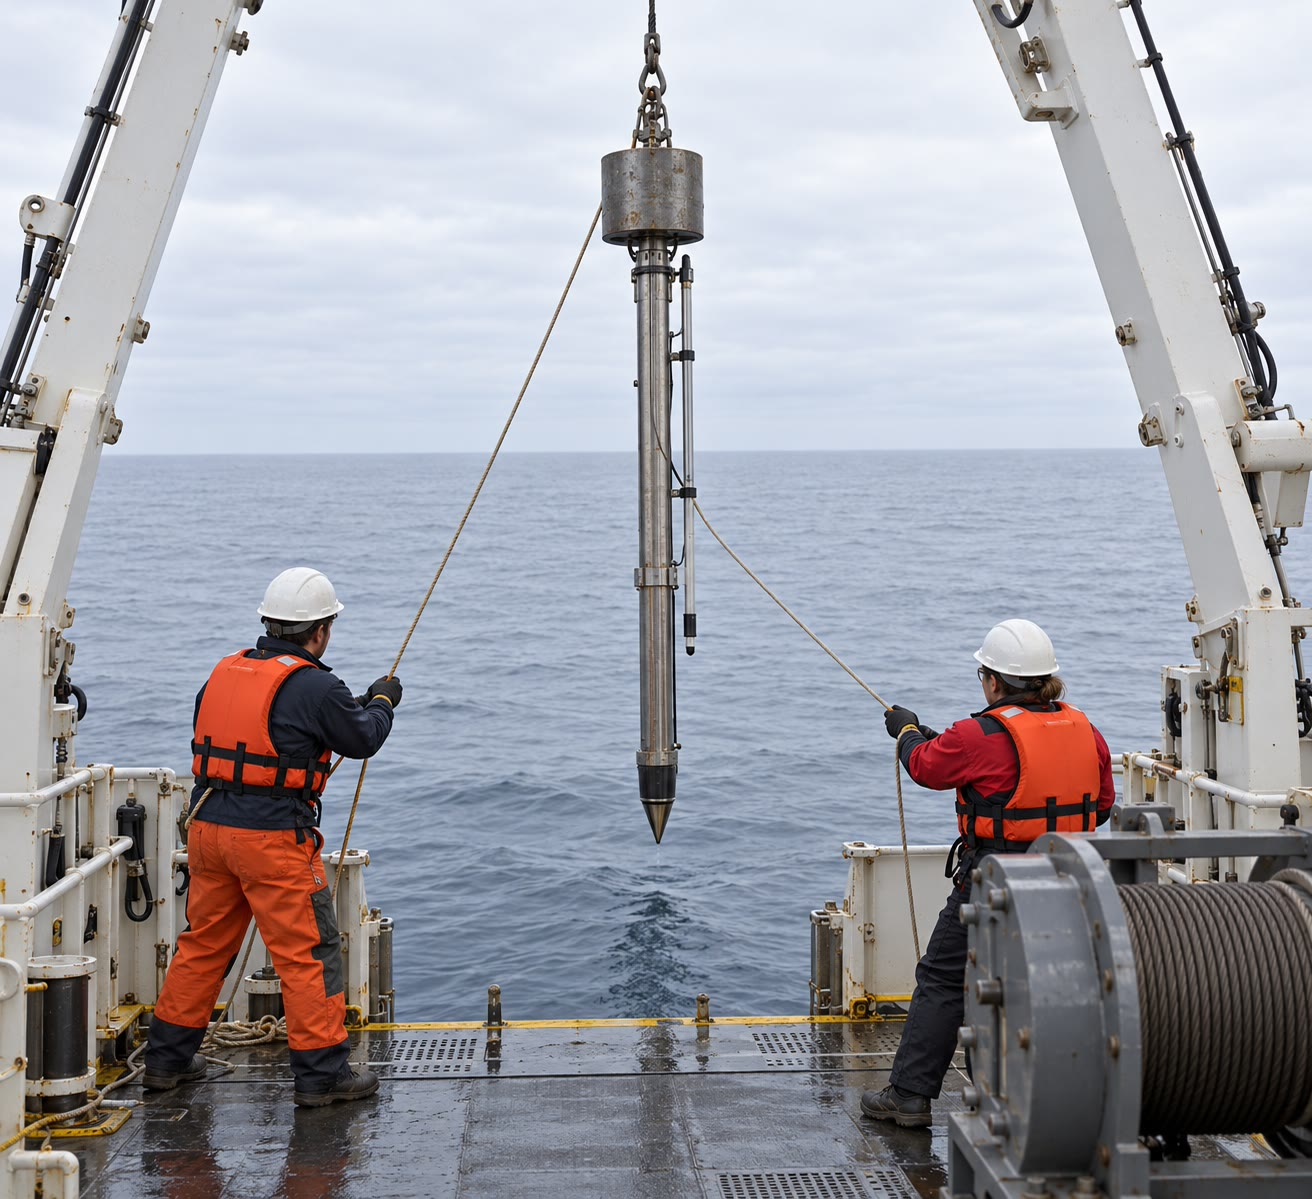
\includegraphics[width=\linewidth]{images/book5/ai/b3-heatflow-probe.jpg}

{\scriptsize رمح قياس التدفق الحراري على وشك أن يُنزل من مؤخرة
سفينة بحث (رسم توضيحي مولَّد بالذكاء الاصطناعي).}
\end{minipage}
\end{inthefield}

\section{التمارين}

\begin{exercise}[$\star$]\label{exo:b3:lithosphere-thermal-models:1}
بفرض $\kappa = \qty{e-6}{m^2.s^{-1}}$، احسب زمن التوصيل $L^2/\kappa$
لقيم $L = 1$، و10، و\qty{100}{km}، محسوبًا بملايين السنين.
\end{exercise}

\begin{exercise}[$\star$]\label{exo:b3:lithosphere-thermal-models:2}
تتعرّض سلسلة جبلية للتعرية بمعدّل \qty{1}{mm/yr}، ويصعد الصخر عبر الجزء العلوي
\qty{30}{km} من القشرة ليعوّض ذلك. بفرض $\kappa = \qty{e-6}{m^2.s^{-1}}$،
احسب عدد بيكليه. هل يمكن حساب المنحنى الحراري للسلسلة بالتوصيل
وحده؟
\end{exercise}

\begin{exercise}[$\star$]\label{exo:b3:lithosphere-thermal-models:3}
في نموذج نصف الفضاء ($T_0 = 0$، $T_m = \qty{1450}{\celsius}$، $\kappa =
\qty{0.8e-6}{m^2.s^{-1}}$)، احسب درجة الحرارة على عمق \qty{10}{km} تحت
قاع بحر عمره \qty{5}{Myr} (علمًا أنّ \qty{1}{Myr} $= \qty{3.156e13}{s}$؛ $\operatorname{erf}
0.445 = 0.471$).
\end{exercise}

\begin{exercise}[$\star$]\label{exo:b3:lithosphere-thermal-models:4}
بفرض $C_q = \qty{490}{mW.m^{-2}.Myr^{1/2}}$، احسب التدفق الحراري عبر
قاع بحر عمره 1 و25 و\qty{100}{Myr}. أيّ هذه الأعمار الثلاثة يُرجَّح أن يقدّر
المسبار التدفق فيه بأقل من قيمته؟
\end{exercise}

\begin{exercise}[$\star\star$]\label{exo:b3:lithosphere-thermal-models:5}
في نموذج نصف الفضاء، تبلغ درجة الحرارة \qty{90}{\percent} من $T_m$
حيث $\operatorname{erf}\eta = 0.9$، $\eta = 1.163$. بفرض $\kappa =
\qty{0.8e-6}{m^2.s^{-1}}$، احسب هذا العمق عند 10 و40 و\qty{100}{Myr}.
\end{exercise}

\begin{exercise}[$\star\star$]\label{exo:b3:lithosphere-thermal-models:6}
بالقيم الواردة في النص، يعطي نموذج نصف الفضاء $C =
\qty{370.5}{m.Myr^{-1/2}}$. مع إبقاء كل القيم الأخرى ثابتة، ما معامل التمدّد الحراري
الذي يعطي القيمة المُلائمة \qty{350}{m.Myr^{-1/2}}؟ وما الوسيط الآخر
الذي يمكن تغييره بدلًا من ذلك؟
\end{exercise}

\begin{exercise}[$\star\star$]\label{exo:b3:lithosphere-thermal-models:7}
احسب التدفق الحراري المقارب $kT_m/L$ لنموذج الصفيحة من أجل $L =
\qty{95}{km}$، $T_m = \qty{1450}{\celsius}$، ومن أجل $L = \qty{125}{km}$،
$T_m = \qty{1350}{\celsius}$، بفرض $k = \qty{3.1}{W.m^{-1}.K^{-1}}$ في الحالتين.
أيُّهما أقرب إلى التدفق الحراري لقاع محيط قديم المحسوب من $C_q/\sqrt t$
عند \qty{150}{Myr} بفرض $C_q = \qty{490}{mW.m^{-2}.Myr^{1/2}}$؟
\end{exercise}

\begin{exercise}[$\star\star$]\label{exo:b3:lithosphere-thermal-models:8}
لدينا إقليم فيه $q_0 = \qty{60}{mW.m^{-2}}$، و$h_r = \qty{10}{km}$، و$A_0h_r =
0.4\,q_0$. احسب $A_0$، و$q_m$، ودرجة الحرارة عند الموهو الواقع
على عمق \qty{35}{km}، بفرض $k = \qty{2.5}{W.m^{-1}.K^{-1}}$.
\end{exercise}

\begin{exercise}[$\star\star$]\label{exo:b3:lithosphere-thermal-models:9}
بلوتونان غرانيتيّان من إقليم واحد يعطيان $q_0 = \qty{66}{mW.m^{-2}}$ مع $A_0
= \qty{3.0}{\micro W.m^{-3}}$، و$q_0 = \qty{48}{mW.m^{-2}}$ مع $A_0 =
\qty{1.2}{\micro W.m^{-3}}$. بافتراض أنّهما يقعان على
\cref{prop:b3:lithosphere-thermal-models:exponential}، احسب $h_r$ و$q_m$.
\end{exercise}

\begin{exercise}[$\star\star\star$]\label{exo:b3:lithosphere-thermal-models:10}
(أ) بيّن أنّ الحرارة المفقودة عبر قاع البحر بين العمرين 0 و$t$، لوحدة
المساحة، هي $Q(t) = 2k(T_m - T_0)\sqrt{t/(\pi\kappa)}$ في نموذج نصف
الفضاء. (ب) بيّن أنّ الهبوط هو $d - d_r = \alpha Q/\bigl(c(\rho_m -
\rho_w)\bigr)$، حيث $c = k/(\rho_m\kappa)$ هي الحرارة النوعية. (ج) تحقّق منه
عدديًا عند \qty{40}{Myr} بالقيم الواردة في النص.
\end{exercise}

\begin{exercise}[$\star\star\star$]\label{exo:b3:lithosphere-thermal-models:11}
في نموذج الصفيحة الوارد في النص ($\tau = \qty{36.2}{Myr}$، $\rho_m\alpha T_mL/
\bigl(2(\rho_m - \rho_w)\bigr) = \qty{3104}{m}$)، العمق المحسوب بحدّ فورييه الأول وحده
يتجاوز المتسلسلة الكاملة أساسًا بفعل الحدّ $n = 3$.
احسب مقدار هذا الحدّ عند 1 و10 و\qty{20}{Myr}، والعمر الذي بعده
يبعد الحدّ الأول وحده عن المتسلسلة بما لا يتجاوز \qty{10}{m}.
\end{exercise}

\begin{exercise}[$\star\star\star$]\label{exo:b3:lithosphere-thermal-models:12}
(أ) بيّن أنّه، في المنحنى الحراري حسب \cref{prop:b3:lithosphere-thermal-models:exponential}،
$T(z) \approx q_mz/k + A_0h_r^2/k$ من أجل $z \gg h_r$. (ب) استنتج عمق
متساوي الحرارة \qty{1300}{\celsius} عند $q_0 = \qty{40}{mW.m^{-2}}$، بالقيم الواردة في
التمرين 8. (ج) بكم ينبغي أن ينخفض $q_m$ حتّى يبلغ ذلك العمق
\qty{250}{km}، عمق الجذور السريعة للكراتونات؟
\end{exercise}

\section{مسألة: أربعون مليون سنة بعيدًا عن الظهرة}

\begin{problem}[{مسألة نهاية الأسبوع --- نصف الفضاء والصفيحة، وعمق محيط
مختلَق، وثخانة صفيحته}]
\label{pb:b3:lithosphere-thermal-models:1}
% values: calc/ch05.py; plate_cooling.py; honda04:gdh1, ps77:depth-age, data:b5-depth-age
خُذ $T_0 = 0$، $T_m = \qty{1450}{\celsius}$، $\kappa =
\qty{0.8e-6}{m^2.s^{-1}}$، $k = \qty{3.1}{W.m^{-1}.K^{-1}}$، $\alpha =
\qty{3.1e-5}{K^{-1}}$، $\rho_m = \qty{3300}{kg.m^{-3}}$، $\rho_w =
\qty{1030}{kg.m^{-3}}$، وظهرة عمقها \qty{2500}{m}، و\qty{1}{Myr} $=
\qty{3.156e13}{s}$.

\medskip\noindent\textbf{الجزء الأول --- نصف الفضاء.}
\begin{enumerate}
  \item احسب $\sqrt{\kappa t}$ عند 10 و\qty{40}{Myr}.
  \item احسب درجة الحرارة على عمق \qty{20}{km} تحت القاع عند العمرين
        ($\operatorname{erf}0.6294 = 0.6266$, $\operatorname{erf}0.3147 =
        0.3437$).
  \item متساوي الحرارة \qty{1000}{\celsius} يقع حيث $\operatorname{erf}\eta =
        0.6897$، $\eta = 0.7174$. احسب عمق هذا المتساوي عند العمرين، والعمر
        الذي يبلغ عنده العمق \qty{60}{km}.
  \item احسب التدفق الحراري عند العمرين، و$C_q$.
  \item تتّسع الظهرة بمعدّل \qty{25}{mm/yr} على كلّ جانب. احسب عدد بيكليه
        للصفيحة عبر \qty{95}{km}. لماذا يجوز أن يُبرَّد كلّ عمود
        على حدة؟
  \item احسب زمن التوصيل عبر \qty{95}{km}. ماذا يقول عن
        نموذج نصف الفضاء لقاع بحر عمره \qty{150}{Myr}؟
\end{enumerate}

\medskip\noindent\textbf{الجزء الثاني --- الهبوط.}
\begin{enumerate}[resume]
  \item تذكّر توازن الإيزوستازيا الذي يحوّل عجز درجة الحرارة في العمود إلى هبوط،
        ولماذا يجوز أخذ التكامل إلى ما لا نهاية
        في نصف الفضاء.
  \item احسب $C$ في قانون العمق والعمر، والعمقين عند 10 و\qty{40}{Myr}.
        \qty{40}{Myr}.
  \item الوسيط لعمق قاع المحيط الحقيقي بين \qty{40}{Myr} و\qty{45}{Myr}
        هو \qty{4475}{m}، دون تصحيح. قارنه بالنموذج عند
        \qty{42.5}{Myr}، واذكر ما يتضمنه الوسيط الذي لا يأخذه
        النموذج في الحسبان.
  \item بكم سيتغيّر $C$ إذا كانت $T_m$ تساوي \qty{1350}{\celsius}؟
        قارنه بالقيمة المُلائَمة \qty{350}{m.Myr^{-1/2}}.
  \item لماذا تقلّ التدفقات الحرارية المقاسة على القاع الفتيّ عن $C_q/\sqrt t$؟
\end{enumerate}

\medskip\noindent\textbf{الجزء الثالث --- الصفيحة.} خذ $L = \qty{95}{km}$.
\begin{enumerate}[resume]
  \item احسب $\tau$ والسعة $\rho_m\alpha T_mL/\bigl(2(\rho_m -
        \rho_w)\bigr)$.
  \item احسب العمق عند \qty{40}{Myr} بالحدود $n = 1$، 3 و5.
  \item بكم يختلف الحدّ الأول وحده عن ذلك، ولماذا
        يكون الاختلاف ضئيلًا؟
  \item احسب الفرق بين نصف الفضاء والصفيحة عند \qty{40}{Myr}
        و\qty{50}{Myr}، وقدّر بالاستيفاء الخطي العمر الذي يبلغ عنده
        الفرق \qty{100}{m}.
  \item احسب التدفق الحراري للصفيحة عند \qty{40}{Myr}، بالحدود
        $n = 1$ إلى 3، وقارنه بنصف الفضاء.
  \item أعطِ العمق المقارب والتدفق الحراري المقارب.
\end{enumerate}

\medskip\noindent\textbf{الجزء الرابع --- محيط متخيَّل.} في محيط متخيَّل
يبلغ عمق ظهرته \qty{2500}{m}، فإنّ القاع، بعد تصحيحه من الرواسب وبعيدًا عن الجبال البحرية والانتفاخات،
يبلغ عمقه \qty{5700}{m} عند \qty{120}{Myr} و\qty{4800}{m} عند \qty{40}{Myr}.
قيمة $L$ للصفيحة غير معلومة، وكل قيمة أخرى
كما سبق.
\begin{enumerate}[resume]
  \item بالاحتفاظ بالحد الأول من متسلسلة فورييه فقط، اكتب العمق عند
        \qty{120}{Myr} دالةً في $L$، مع اعتماد $\tau$ نفسه على
        $L$.
  \item حُلَّ المعادلة لإيجاد $L$ بالتكرار، ابتداءً من $L = \qty{100}{km}$:
        احسب $\tau$، ثم $L$ الذي يطابق \qty{5700}{m} بهذه
        $\tau$، وكرّر.
  \item مع $L$ الذي وجدته، احسب العمق عند \qty{40}{Myr}، وقارنه
        بنصف الفضاء وبالقيمة المقاسة \qty{4800}{m}.
  \item احسب $\tau$ لهذا $L$ والعمق المقارب لهذا المحيط.
  \item بعد أيّ عمر يقع القاع ضمن \qty{100}{m} من
        عمقه المقارب؟
  \item أعطِ سمك الصفيحة $L$ الذي يلائم القاع القديم للمحيط
        المتخيَّل.
\end{enumerate}
\end{problem}
